\documentclass[11pt,a4paper,openany]{book}
\usepackage[utf8]{inputenc}
\usepackage[T1]{fontenc}
\usepackage[spanish]{babel}
\usepackage{amsmath}
\usepackage{amsfonts}
\usepackage{amssymb}
\usepackage{graphicx}
\author{Henrri Quino Huerta}
\title{monografia}
%%%%%%%%%%%%%%%%%%%%%%%%%%
\usepackage[left=2.54cm,right=2.54cm,top=2.54cm,bottom=2.54cm]{geometry}
\usepackage{float}
\usepackage{setspace}
\usepackage[colorlinks=true,linkcolor=black,urlcolor=blue]{hyperref}
\newtheorem{obs}{Observación}[section]
\newtheorem{teorem}{Teorema}[section]
\usepackage{url}
%%%%%%%%%%%%%%%%%%%% para introducir codigo Matlab
\usepackage{listings}
\usepackage{color}
\usepackage{textcomp}
\lstset{
	tabsize=4,
	rulecolor=,
	basicstyle=\scriptsize,
	upquote=true,
	aboveskip={1.5\baselineskip},
	columns=fixed,
	showstringspaces=false,
	extendedchars=true,
	breaklines=true,
	prebreak = \raisebox{0ex}[0ex][0ex]{\ensuremath{\hookleftarrow}},
	showtabs=false,
	showspaces=false,
	showstringspaces=false,
	identifierstyle=\ttfamily,
	keywordstyle=\color[rgb]{0,0,1},
	commentstyle=\color[rgb]{0.133,0.545,0.133},
	stringstyle=\color[rgb]{0.627,0.126,0.941},
}
\begin{document}
		\frontmatter
		\begin{titlepage}
	\begin{center}
		{\LARGE \textbf{Universidad Nacional Mayor de San Marcos}}\\
		\vspace{0.25cm}
		{\large \textbf{Universidad del Perú. Decana de América}}
		\begin{figure}[H]
			\centering
			
\includegraphics[scale=0.6]{caratula/unmsm.pdf}
		\end{figure}
		\rule{150mm}{0.2mm}
		\begin{spacing}{2}
			
			{\Large \textbf{La ecuación de Fisher-Kolmogorov en oncología}}\\
			
			{\Large \textbf{Simulación numérica}}
		\end{spacing}
		\rule{150mm}{0.6mm}
		
		\vspace{2cm}
		{\LARGE \textbf{Facultad de Ciencias Matemáticas}}
		
		\vspace{5mm}
		{\Large \textbf{EAP Matemática}}
		
		\vspace{5mm}
		{\Large \textbf{Matemática Computacional II}}\\
		
		\vfill
		{\Huge 2020}
	\end{center}
\end{titlepage}

 
		\chapter*{Integrantes del grupo}
		\begin{enumerate}
	\item Arakawa Yagi Patricia - $07140128$
	\item Avendaño Rodriguez Alexander - $14140174$
	\item Baltazar Rico Mayumi Alejandra - $12140144$
	\item Borja Ayala Bruno Antony - $17140008$
	\item Davalos Cámac Gabriel Alonso - $16140116$
	\item De la Cruz De la Cruz Wiliam Davis - $09140150$
	\item Montalvo Olazabal Jesús Fernando - $17140037$
	\item Quino Huerta Henrri Wilmer - $17140023$
	\item Valencia Chávez Frank Leonel - $17140131$
\end{enumerate}
		\tableofcontents
		\mainmatter
		\chapter*{Introducción}
		En la actualidad el \textit{Cáncer} es una de las palabras que más asusta cuando se habla de salud, ya que no se trata únicamente de una enfermedad sino que este término hace referencia a muchas enfermedades que tienen un denominador común: la transformación de la células normales en células cancerosas las cuales se dividen sin control y pueden invadir otros tejidos.\\

En la literatura existen numerosos modelos matemáticos que intentan describir  procesos que ocurren durante el desarrollo del cáncer, algunos de estos decriben: el crecimiento de tumores cancerosos, la respuesta del sistema inmune a la presencia de células cancerosas en el cuerpo, movimiento de las células cancerosas y su propagación en el organismo, control de crecimiento de tumores, modelos de vascularización o angiogénesis de los mismos, entre otros.\\

El estudio  matemático que presentaremos busca en concreto modelar tumores cerebrales. Para ello haremos uso de las ecuaciones en derivadas parciales que nos permitirá introducir un primer modelo sencillo en la cual nuestro principal objetivo es hacer un análisis y solución numérica del modelo aplicado a un caso concreto, gliomas, para el cual haremos uso de Matlab.
		\chapter{Marco teórico}
		El presente trabajo pretende exhibir un modelo matemático en EDP(Ecuaciones en derivadas parciales) que pueda predecir el crecimiento de un tumor cerebral a lo largo del tiempo; para dar la expresión explícita del modelo (ecuaciones), necesitamos partir de algunos conceptos y modelos previos.\\

%%%%%%%%%%%%%%%%%%%%%%%%%%%%%%%%%%%%%%%%%%%%%%%%%%%%%%%%%%%%%%%%%%%%%%%%%%%%%%%%%%%%%%%%%%%%%%% 
\section{¿Qué es el cáncer?}

\subsection{Antecedentes}

En la antig\"uedad el hombre no estaba menos preocupado por la prevención y cura de enfermedades como ocurre ahora; sin embargo,
diversas entidades como cultos y santuarios, e incluso profesionales dedicados a la salud punteaban los paisajes espirituales, físicos y
profesionales del mundo antiguo.\\

Especialidades de distintas ramas como arqueología, paleontología y paleomedicina han descubierto en diversas culturas restos óseos humanos fosilizados afectados por el cáncer y han determinado su antig\"uedad en miles de años atrás mediante carbono $14$.\\

Ese descubrimiento fue importante pues nos hace asegurar que incluso en el pasado ha existido el cáncer y que en la actualidad se ha configurado en la principal causa de muerte en todo el mundo.

\subsection{¿Qué sabemos del cáncer en la actualidad?}

Sabemos que nuestro organismo está constituido por un gran número de células y que estas son la unidad anatómica fundamental funcional de todos los seres vivos y además su composición es compleja y única, como por ejemplo: el ADN y el ARN.\\

Cada una de las células crece y se divide de manera coordinada y ordenada; sin embargo, algunas veces este proceso se descontrola y el material genético contenido en el ADN se daña o se altera, provocando así mutaciones irreversibles que afectan en el crecimiento y la división normal de las células.\\

Cuando esto último sucede, las células no mueren cuando deberían morir, y se forman células nuevas a pesar de que el cuerpo no las necesita y estas forman una masa de tejido a la que se le llama \textbf{tumor}.

\subsection{Definición}

Se le llama \textbf{cáncer} cuando el tumor es maligno y tiene la capacidad de invasión, infiltración y de producir metástasis a lugares distantes del tumor primario. No obstante, no todos los tumores son cancerosos, entre ellas tenemos:
 
\begin{itemize}
	\item \textbf{Tumores benignos}: Son aquellos que pueden extirparse y en la mayoría de los casos no vuelven a aparecer. Las células no se diseminan a otras partes del cuerpo.
	\item \textbf{Tumores malignos}: Son aquellos en las que las células pueden invadir tejidos cercanos y diseminarse a otras partes del cuerpo.
\end{itemize}

Al proceso en el que las células cancerosas se desprenden del tumor original y viajan a través de la sangre o el sistema linfático y forman un tumor nuevo en otros órganos o tejidos se le llama \textbf{metástasis}.
\subsection{Causas}

El proceso por el cual se produce el cáncer es causado por anormalidades en el material genético de las células. Estas anormalidades pueden ser ocasionadas por:

\begin{itemize}
	\item Agentes carcinógenos como las irradiaciones. 
	\item Algunos productos químicos como el humo del tabaco y el humo de leña.
	\item Por agentes infecciosos como el VIH y el de la hepatitis B.
	\item Anormalidades genéticas adquiridas durante la replicación del ADN.
\end{itemize} 
\subsection{Clasificación}

Por lo general el cáncer se clasifica según los órganos o tejidos en donde se presenta y también se describe según el tipo de célula por el que está formado.

\begin{itemize}
	\item \textbf{Carcinoma}: cáncer que empieza en la piel o en los tejidos que cubren órganos internos.
	\item \textbf{Sarcoma}: cáncer que empieza en el hueso, cartílago, grasa, músculo o vasos sanguineos.
	\item \textbf{Leucemia}: cáncer que empieza en el tejido en el que se forma la sangre, como la médula ósea.
	\item \textbf{Linfoma y mielioma}: cáncer que empieza en las células del sistema inmunitario
	\item \textbf{Cáncer del sistema nervioso central}: cáncer que empieza en los tejidos del cerebro y la médula espinal.
\end{itemize}

Los cinco tipos de cáncer que causan un mayor número de fallecimientos son los siguientes:

\begin{itemize}
	\item Pulmonar
	\item Hepático
	\item Colorrectal
	\item Gástrico
	\item Mamario
\end{itemize}

\subsection{Tumores cerebrales}

Estos tumores se pueden originar a partir de las células cerebrales, las membranas alrededor del cerebro, nervios o glandulas. Los tumores pueden destruir directamente células cerebrales o provocarles daño produciendo inflamación, ejerciendo presión sobre otras partes del cerebro e incrementando la presión intracraneal.\\

Los tumores cerebrales pueden ocurrir a cualquier edad, pero muchos de ellos son más comunes en un grupo de edad en particular. Por ejemplo, en los adultos, los gliomas y los meningiomas son los más comunes.\\

Los \textit{meningiomas} son muy frecuentes y por lo general benignos.No obstante pueden causar serias complicaciones e inluso la muerte debido a su tamaño y localización.\\

Por el contrario los \textit{gliomas},a pesar de que apenas metastatizan, rara vez se pueden curar. Surgen a partir de las células gliales,es decir, células del sistema nervioso central que desempeñan de forma principal, la función de soporte de las neuronas e intervienen activamente en el procesamiento cerebral de la información en el organismo. Son clasificados de acuerdo a su grado, y del cual depende que se augure un mejor o un peor pronóstico, siendo éste por lo general malo para pacientes con gliomas de alto grado.\\

Esta presente investigación tiene como objetivo encontrar una ecuación en derivadas parciales con las condiciones necesarias que modele en concreto los gliomas y resolverla empleando el método numérico adecuado.\\

\begin{figure}[H]
	\centering
	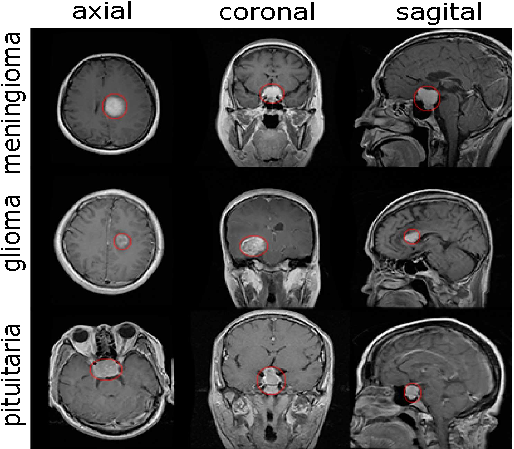
\includegraphics[scale=1.2]{marcoteorico/tumorcerebral.pdf}			
	\caption{{\small {\footnotesize Representación de imágenes de resonancia magnética (MRI) normalizadas que muestran diferentes tipos de tumores en diferentes planos. En las imágenes, el tumor está marcado con un contorno rojo. El ejemplo se da para cada tipo de tumor en cada uno de los planos.}}}
\end{figure}

\newpage
%%%%%%%%%%%%%%%%%%%%%%%%%%%%%%%%%%%%%%%%%%%%%%%%%%%%%%%%%%%%%%%%%%%%%%%%%%%%%%%%%%%%%%%%%%%%%%%%
\section{Ecuación de Reacción-Difusión.}\label{cap: Ec Re Dif}
Estas ecuaciones son importantes en derivadas parciales e implican la combinación de dos procesos diferentes: \textit{reacción} y \textit{difusión}. Empecemos definiendo estos dos conceptos:
\begin{itemize}
	\item \textbf{Difusión}: Es la tendencia de las moléculas a moverse desde zonas de alta concentración hacia zonas de baja concentración.
	\item \textbf{Reacción}: Se entiende como el cambio de estado de las partículas debido por ejemplo a interacciones o de manera espontánea.
\end{itemize}
Estas ecuaciones se sitúan en el campo del Modelado Matemático de Sistemas Biológicos, y se debe tener en cuenta que este modelo surge para intentar describir un medio(sistema) que ignora por completo el efecto de las fluctuaciones internas(algo común en cualquier sistema discreto). A pesar de ello, tales fluctuaciones pueden provocar cambios drásticos en la dinámica, lo que ocasiona una ruptura de las aproximaciones que se obtengan del sistema. Los casos más complejos, se han estudiado en trabajos que incorporan métodos estocásticos.\\

Cabe mencionar que este modelo se ha estudiado sobre todo en dominios espaciales estáticos, sin embargo en los sistemas biológicos es común encontrar dominios en crecimiento; en particular el interés de los dominios en crecimiento se hace evidente en la biología del desarrollo, donde una característica común de los sistemas estudiados es su tamaño dependiente del sistema.\\

Por todo lo expuesto anteriormente, en años recientes, este modelo para dominios en crecimiento viene siendo objeto de gran interés en investigación biológica.\\

Esta ecuación comprende dos factores importantes, uno de difusión y otro de reacción, y el modelo es el siguiente:

\begin{equation}
	\label{ReaccionDifusion1}
	{ u }_{ t }=d\triangle u+f(u)
\end{equation}

\vspace{0.2cm}
Donde:

\begin{itemize}
	\item $u(x,t)$ es la variable de estado y describe la densidad(concentración) de una sustancia(población) en la posición $ x\in \Omega\subset { \mathbb{R} }^{ n }$ y en el instante $t $. (Tener en cuenta que $\Omega$ es un conjunto abierto). Además el operador $ \triangle $ es el Laplaciano.
	\item El factor $d\triangle u $ describe la difusión del sistema, siendo $d$ el coeficiente de difusión.
	\item El factor $f(u)$ es una función suave $f:\mathbb{R}\rightarrow \mathbb{R} $, y este describe el proceso con el que realmente cambia $u$; es decir, podría ocurrir un proceso como nacimiento, muerte,reacción química, etc.
\end{itemize}

Entendiéndose en términos más simples, el \textbf{factor de difusión} nos dice qué tanto cambia el espacio (expande o contrae) y \textbf{el factor de reacción} nos da información acerca de lo que pasa dentro del espacio y los cambios que ocurren en él. Obteniendo así información del sistema completo.\\

Este modelo se puede llevar a sistemas más complejos en los que el factor de Reacción no solo dependa de $u$, sino también de su derivada($ \nabla u$) o incluso de la variable espacial $x$, en tal caso tendríamos lo siguiente:

\begin{equation}
	\label{ReaccionDifusion2}
	 u_{ t }=d\triangle u + f(x,u,\nabla u)
\end{equation}

\vspace{0.2cm}
Sin embargo, para este trabajo solo tomaremos la idea de la ecuación (\ref{ReaccionDifusion1})
%%%%%%%%%%%%%%%%%%%%%%%%%%%%%%%%%%%%%%%%%%%%%%%%%%%%%%%%%%%%%%%%%%%%%%%%%%%%%%%%%%%%%%%%%%%%%%%
\section{Modelo logístico de poblaciones.}\label{cap:mod log pob}
Los dos modelos más simples de crecimiento poblacional utilizan ecuaciones determinísticas(ecuaciones que no consideran los eventos aleatorios) para describir la tasa de cambio en el tiempo de la población. El primero de estos , \textbf{crecimiento exponencial}, describe poblaciones que incrementan su número sin ningún límite; sin embargo esto solo es posible  únicamente cuando hay disponible una cantidad infinita de recursos, lo cual no ocurre en la realidad ya que si los individuos se incrementan los recursos se terminaran, la tasa de crecimiento disminuirá. Eventualmente la tasa de crecimiento alcanzará una asíntota o se estabilizará. Este tamaño de la población, que esta determinado por un tamaño máximo de población que un ambiente puede mantener se llama \textbf{capacidad de carga}. Por tanto en este segundo caso se dice que la población tiene un \textbf{crecimieno logístico}. 

\begin{center}
	\begin{figure}[H]
		\centering
		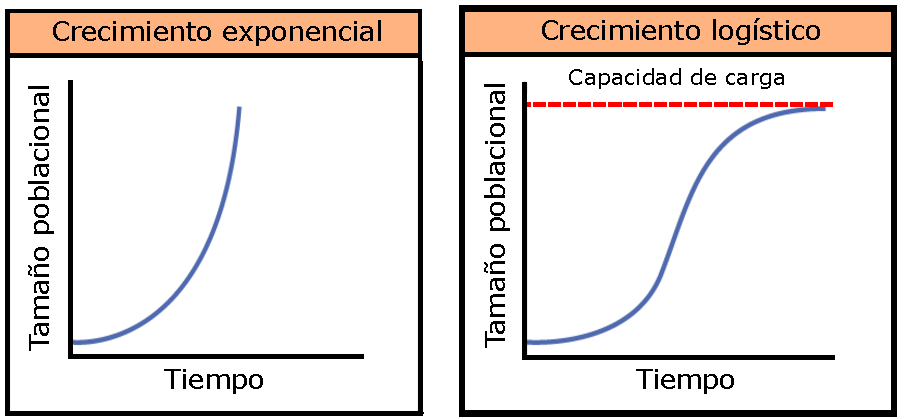
\includegraphics[scale=1]{marcoteorico/crecimientologistico.pdf}			
		\caption{{\small {\footnotesize Dos modelos básicos que describen el crecimiento poblacional}}}
	\end{figure}
\end{center}

Si bien, existen muchos modelos matemáticos más sofisticados sobre poblaciones de organismos biológicos, el siguinte modelo en particular será de sumo interés pues será este quien nos conducirá a la ecuación medular de este trabajo(Ecuación de Fisher-Kolmogorov)\\

Si usamos un modelo poblacional, en el que se asume que los recursos son limitados tendremos el siguiente sistema:

\begin{equation}
	\label{Logistico5}
	\begin{cases} u'(t)=\rho u(t)\left[ A-u(t) \right]  \\ u(0)={ f }_{ 0 }\quad ;{ \quad f }_{ 0 }\in \left( 0,A \right) \quad  \end{cases}
\end{equation}\\

Donde $u(t)$ es la densidad de población; $\rho>0 $ es el índice de crecimiento y $A>0$ es llamada Capacidad de Carga del Ambiente.\\

Este sistema (\ref{Logistico5}) se puede resolver fácilmente, solo usando el método de Separación de Variables, llegando al siguiente resultado:

\begin{equation}
	\label{Logistico6}
	u(t)=\dfrac { A{ f }_{ 0 } }{ { f }_{ 0 }+(A-{ f }_{ 0 }){ e }^{ -\rho At } } \quad ;t\ge 0
\end{equation}

Un detalle curioso para esta ecuación es que si: $ t\rightarrow \infty \Rightarrow { e }^{ -\rho At }\rightarrow 0\Rightarrow u(t)\rightarrow A$\\

Esto nos dice que $u(t)=A$ es la solución asintótica para cualquier valor inicial ${ f }_{ 0 }>0$. Esto explica el porqué, $A$ recibe el nombre de Capacidad de Carga del Ambiente, pues es el valor máximo alcanzable(población en un tiempo suficientemente grande)
%%%%%%%%%%%%%%%%%%%%%%%%%%%%%%%%%%%%%%%%%%%%%%%%%%%%%%%%%%%%%%%%%%%%%%%%%%%%%%%%%%%%%%%%%%%%%%%%%%%%%%%%%%%
\section{Deducción de las ecuaciones de Reacción-Difusión}
En la sección \ref{cap: Ec Re Dif} se habló acerca de la ecuación de Reacción-Difusión, y los conceptos relacionados a estos dos términos e incluso se presentó su forma general (la ecuación \eqref{ReaccionDifusion2}); sin embargo, no se dio justificaciones al respecto; ahora pretendemos desglosar algunos detalles.\\

Se supone una población $u(x,t)$ en un conjunto $\Omega \subset \mathbb{R}^n$ abierto y se denota por $ J(x,t) \in \mathbb{R}^n$ el flujo de partículas que entran y salen de $\Omega$.\\

La \textbf{ecuación de conservación} nos dice que \textit{la tasa de cambio de la densidad $u(x,t)$ en $\Omega$ es igual a la tasa de cambio del flujo del material a través de $\partial \Omega$ más el material creado en $\Omega$}.\\

Es decir:

\begin{center}
	\begin{tabular}{c c c}
		CAMBIO EN $\Omega \quad = $ & FLUJO A TRAVÉS DE $\partial\Omega$ & $+\quad$ CAMBIO EN LA TASA DE  \\
	 	 &  & NACIMIENTO Y MUERTE EN $\Omega$ \\
	\end{tabular}
\end{center}

Matemáticamente:\\

\begin{equation}
	\dfrac { \partial  }{ \partial t } \int _{ \Omega  }{ u(x,t)d\Omega  } =-\int _{ \partial \Omega  }{ J(x,t)\cdot \vec {n}\, d\,\partial \Omega } +\int_{ \Omega}\,{ f(u(x,t))\,d\Omega }
	\label{eq:reacdifintegral}
\end{equation}\\

donde $f(x,t)$ describe la tasa de nacimiento, muerte, etc. Notar, que consideramos que al final la tasa media del flujo entra.

\begin{teorem}[\textbf{Teorema de la divergencia de Gauss }]\label{teoremaGaus}
	\upshape{Sea $\Omega$ un abierto de $\mathbb{R}^2$ y $S = \partial \Omega$ su borde, orientado con la norma exterior unitaria $\vec{n}$. Sea $F : \Omega \rightarrow \mathbb{R}^2$ un campo vectorial de clase $C^1(\Omega)$. Entonces:
		
		$$\int_\Omega divF d\Omega=\int_S F\cdot \vec{n}dS $$
	}
\end{teorem}

 De esta manera, haciendo uso del teorema \ref{teoremaGaus} y sustituyendo en la ecuación \eqref{eq:reacdifintegral} se obtiene la siguiente igualdad:
 
 \begin{equation}
 	\int_\Omega \left(\frac{\partial u}{\partial t} - f(u) + divJ\right)d\Omega = 0
 	\label{eq:gauscero}
 \end{equation}

 Luego, por la \textbf{ley de Fick}, el flujo es proporcional al gradiente de la concentración del material; es decir:
 
$$ J = -d\bigtriangledown u $$

donde $d$ es el \textit{coeficiente de difusión} y el signo negativo es debido al hecho de que va de mayor a menor densidad.\\

Así reemplazando $J$ en la igualdad \eqref{eq:gauscero} se llega a la siguiente ecuación.

$$ \frac{\partial u}{\partial t} = \bigtriangledown(d\bigtriangledown u) + f(u)$$

Operando esta última expresión obtendremos la \textbf{ecuación de Reacción-Difusión} dada en la sección \ref{cap: Ec Re Dif}.

\begin{equation}
	\label{deduccion3}
	\dfrac { \partial u(x,t) }{ \partial t } =d\Delta u(x,t)+f(u(x,t))\quad ;(x,t)\in \Omega\times { \mathbb{R} }^{ + }
\end{equation}

\vspace{0.1cm}
\begin{obs}
	\upshape{Nótese además que (\ref{deduccion3}); es decir, $ d{ u }_{ xx }-{ u }_{ t }+f=0$ hace referencia a una \textit{EDP parabólica} pues si identificamos términos con: $a{ u }_{ xx }+b{ u }_{ xt }+c{ u }_{ tt }+d{ u }_{ x }+e{ u }_{ t }+f=0$ tenemos: 
		$$  a=d;\,b=0;\,c=0\quad \quad \Longrightarrow { \quad b }^{ 2 }-4ac={ 0 }^{ 2 }-4(d)(0)=0$$
	}
\end{obs}

A partir de esta ecuación (\ref{deduccion3}) podemos obtener diversos casos, dependiendo de las hipótesis que se quieran tomar en consideración(esto hace que cambie el $f(u)$); por ejemplo:
\begin{enumerate}
	\item Si eliminamos el factor de Reacción, entonces solo tendremos difusión, siendo la ecuación correspondiente, la ecuación del calor ($ { u }_{ t }=d{ u }_{ xx }$)
	
	\item Otro caso más especial es cuando $ f(u)=u(1-{ u }^{ 2 })$, obteniendo así la ecuación de Newell-Whitehead-Segel para describir la convección de Bernard.
	
	\item Otro ejemplo interesante ocurre cuando $ f(u)=u(1-{ u })(u-\alpha )\quad ;0<\alpha <1$; con el cual obtenemos la ecuación de Zeldovich que surge en la teoría de la Combustión.
	
	\item Si $f(u)=u(1-u) $, obtenemos la \textbf{ecuación de Fisher}, usada originalmente para describir la expansión de las poblaciones biológicas.
\end{enumerate}
Este último formará la piedra angular del presente trabajo, la \textbf{ecuación de Fisher-Kolmogorov}; que en su forma más generalizada adopta la expresión:

\begin{equation}
	\label{deduccion4}
	f(u)=\rho u(A-u)\quad \Rightarrow { u }_{ t }=d{ u }_{ xx }+\rho u(A-u)
\end{equation}

donde $d:$ coeficiente de difusión; $\rho: $ parámetro de proliferación; y $A:$ Capacidad del ambiente.\\

\begin{obs}
	\upshape{Nótese la similitud entre lo expuesto en la Sección \ref{cap:mod log pob}, es decir comparemos la expresión (\ref{Logistico5}) y la expresión (\ref{deduccion4}). Esto sucede pues, (\ref{deduccion4}) nace a partir de (\ref{Logistico5}), con el único cambio de que se añade una variable más(espacial) y este está ligado al \textit{factor de difusión }(el espacio se contrae o expande).
	}
\end{obs}
		\chapter{Formulación de la aplicación y método de solución}
		%%%%%%%%%%%%%%%%%%%%%%%%%%%%%%%%%%%%%%%%%%%%%%%%%%%%%%%%%%%%%%%%%%%%%%%%%%%%%%%%%%%%
\section{Ecuación de Fisher-Kolmogorov (FK) en oncología.}

Tal como se mencionó en la \textit{Introducción}, existe una multitud de estudios y modelos matemáticos relacionados al cáncer. El objetivo ahora, es establecer las condiciones hipotéticas para el modelo del crecimiento de un tumor cerebral y ver cómo se acondiciona a la ecuación de Fisher-Kolmogorov (\ref{deduccion4}) , estableciendo así un modelo matemático la cual estudiaremos empleando métodos numéricos\\

Trabajaremos con condiciones de frontera \textit{(Neumann)}, puesto que se asume que el \textit{área es cerrada}, esto para asegurar que no existirá migración de células a través del dominio establecido. Entonces:

\begin{equation}
	\label{oncologia1}
	\dfrac{\partial u(0,t)}{\partial x}=\dfrac{\partial u(L,t)}{\partial x}=0
\end{equation}

\vspace{0.5cm}
donde $L:$ Longitud del dominio. Nótese ademas que solo estamos trabajando en $ \Omega \subset \mathbb{R}$\\

Para esclarecer la frase \textit{área cerrada} podemos mencionar que la principal razón de porqué elegimos este modelo y condiciones de frontera para el estudio de un tumor cerebral(glioma maligno) es que este fenómeno en particular casi siempre presenta ausencia de metástasis.

\begin{obs}
	\upshape{La metástasis ocurre cuando las células cancerosas se separan del tumor original(primario) y viajan a través de la sangre hacia otros órganos y/o tejidos, y forman nuevos tumores. La \textit{ausencia de Metástasis en el tumor cerebral} significa que si se tiene un tumor cerebral, este raramente se expandirá hacia otros órganos, podemos interpretar esto entonces como si tuviéramos una cierta cantidad de puntos en un dominio $ \Omega$ y este sufrirá escasa alteración, al menos por migración de células en todo el dominio.
	}
\end{obs}

También debemos notar que no se está tomando en cuenta la posición de las células en un lugar específico(en qué parte del cerebro), en la realidad esto suele ocasionar grandes variantes, pues nos daría información acerca de la capacidad de invasión y aparente borde del tumor.\\

No obstante, como en todos los tumores, los aspecto biológicos y clínicos de los gliomas, son complejos y los detalles de sus crecimiento espacio-temporal todavía no se entienden bien. Para construir estos modelos buscamos describir los aspectos más básicos  de los gliomas, haciendo uso de la ecuación de Fisher-Kolmogorov para describir la dinámica espacio-temporal de una densidad de células cancerígenas. En la ecuación \eqref{deduccion4} el factor $f(u)$ modela la proliferación, es decir, otorga información acerca del nacimiento y muerte de células cancerosas. Por otro lado, el factor $ d{ u }_{ xx }$ surge a partir de que las células crecen lo suficiente y luego migran, esto es, se difunden.\\

En conclusión, la \textbf{ecuación de Fisher-Kolmogorov (FK)} para el modelo matemático que estima el crecimiento de las células cancerígenas en un tumor cerebral(glioma maligno) es: 

\begin{equation}
	\label{eq: jisus}
	\displaystyle \begin{cases} { u }_{ t }=d{ u }_{ xx }+\rho u(A-u) \\ u(x,0)=g(x) \\ { u }_{ x }(0,t)={ u }_{ x }(L,t)=0 \end{cases}
\end{equation}
%%%%%%%%%%%%%%%%%%%%%%%%%%%%%%%%%%%%%%%%%%%%%%%%%%%%%%%%%%%%%%%%%%%%%%%%%%%%%%%%%%%%%%%%%%%%%%
\section{Esquemas de diferencias finitas para el método de Fisher.}\label{diferenaciasfinitas}

En esta sección estudiaremos los esquemas en diferencias finitas para el sistema \eqref{eq: jisus}. Usaremos las fórmulas de aproximaxión que se pueder ver en el anexo. Partimos de la ecuación:

	$$u_{_{t}}=du_{_{xx}}+\rho(A-u)u$$

Usando diferencias centradas de segundo orden en la variable espacial para aproximar la derivada de segundo orden obtenemos: 

$$u_{_{xx}}(x_{_{i}},t_{_{j}})\simeq\frac{w_{_{i+1,j}}-2w_{_{i,j}}+w_{_{i-1,j}}}{h^{2}}$$

y usando ahora diferencias progresivas en el tiempo para aproximar la derivada de primer orden producimos la siguiente aproximación:

$$u_{_{t}}\simeq\frac{w_{_{i,j+1}}-w_{_{i,j}}}{k}$$

Sustituyendo esas aproximaciones en la ecuación obtenemos la ecuación aproximada:

$$\dfrac{w_{_{i,j+1}}-w_{_{i,j}}}{k}=d\left(\dfrac{w_{_{i-1,j}}-2w_{_{i,j}}+w_{_{i+1,j}}}{h^{2}}\right)+\rho(A-w_{_{i,j}})w_{_{i,j}}$$

Multiplicando ambos lados de la igualdad por $k$, se obtiene

$$w_{_{i,j+1}}-w_{_{i,j}}=\frac{dk}{h^{2}}(w_{_{i-1,j}}-2w_{_{i,j}}+w_{_{i+1,j}})+k\rho(A-w_{_{i,j}})w_{_{i,j}}$$

De donde se tiene:

\begin{equation}
	w_{_{i,j+1}}=w_{_{i,j}}+\sigma(w_{_{i-1,j}}-2w_{_{i,j}}+w_{_{i+1,j}})+k\rho(A-w_{_{i,j}})w_{_{i,j}}
	\label{iteracionsinneumann}
\end{equation}


donde $\sigma=\frac{dk}{h^{2}}$; $h=\frac{L}{m}$ y $k=\frac{T}{n}$ son los tamaños de paso siendo $L$ la longitud del intervalo espacial, $T$ el tiempo final, $m$ y $n$ la cantidad de intervalos en las que se divide el intervalo espacial y temporal respectivamente. Se está considerando $i=0,...,m$ y $j=0,...,n$ \\

Además de la condición de Neumann para $i=0$ aplicando una aproximación progresiva se tiene que:

\begin{equation}
	w_{_{0,j+1}}=w_{_{0,j}}+\frac{dk}{h^{2}}(2w_{_{1,j}}-2w_{_{0,j}})+k\rho(A-w_{_{0,j}})w_{_{0,j}}
	\label{neumannizquierdo}
\end{equation}

Por otro lado haciendo una aproximación centrada de la condición de  Neumann para $i=n$ se tiene:

\begin{equation}
	w_{_{m,j+1}}=w_{_{m,j}}+\frac{dk}{h^{2}}(2w_{_{m-1,j}}-2w_{_{m,j}})+k\rho(A-w_{_{m,j}})w_{_{m,j}}
	\label{neumannderecha}
\end{equation} 

De las ecuaciones \eqref{iteracionsinneumann}, \eqref{neumannizquierdo}, \eqref{neumannderecha} y de la condición inicial tenemos la fórmula de recursividad para aproximar o dar solución numérica al sistema \eqref{eq: jisus}

\subsection{Fórmula recursiva para le ecuación FK}

\begin{equation}
	\label{formularecursiva}
	\displaystyle \begin{cases} w_{_{i,j+1}}=w_{_{i,j}}+\sigma(w_{_{i-1,j}}-2w_{_{i,j}}+w_{_{i+1,j}})+k\rho(A-w_{_{i,j}})w_{_{i,j}}; \,\,1\leq i<m
		
	\vspace{0.5cm} \\
	
	w_{_{0,j+1}}=w_{_{0,j}}+\sigma(2w_{_{1,j}}-2w_{_{0,j}})+k\rho(A-w_{_{0,j}})w_{_{0,j}}
	
	\vspace{0.5cm} \\
	
	
	\vspace{0.5cm}
	w_{_{n,j+1}}=w_{_{n,j}}+\sigma(2w_{_{n-1,j}}-2w_{_{n,j}})+k\rho(A-w_{_{n,j}})w_{_{n,j}}\\
	
	w_{_{i,0}}=g(x_i)\quad 0\leq i\leq m
	\end{cases}
\end{equation}

El siguiente capítulo haremos un programa en Matlab del sistema \eqref{formularecursiva}\\

También podemos expresar \eqref{formularecursiva} dando una forma de iteración matricial. Antes debemos expresar \eqref{iteracionsinneumann} como $$w_{_{i,j+1}}=\sigma w_{_{i-1,j}}+(1-2\sigma)w_{_{i,j}}+\sigma w_{_{i+1,j}}+k\rho(A-w_{_{i,j}})w_{_{i,j}}$$

Luego también considerando \ref{neumannizquierdo} y \eqref{neumannderecha} se tiene:

$$
\begin{bmatrix} 
	w_{_{1,j+1}} \\
	w_{_{2,j+1}} \\
	\vdots\\
	w_{_{m-2,j+1}}\\
	w_{_{m-1,j+1}}
\end{bmatrix}=\begin{bmatrix}
	1-2\sigma  & \sigma    &           &        &      &  &  & \\
	\sigma     & 1-2\sigma & \sigma    &        &      &  &  &  \\
	& \sigma    & 1-2\sigma &\sigma  &      &  &  &  \\
	&           &           &        &\ddots&  &  &  \\
	&           &           &        &\sigma&1-2\sigma&\sigma\\     
	&           &           &        &      &\sigma   &1-2\sigma\\ 			  		     	
\end{bmatrix}\begin{bmatrix}
	w_{_{1,j}} \\
	w_{_{2,j}} \\
	\vdots\\
	w_{_{m-2,j}}\\
	w_{_{m-1,j}}
\end{bmatrix}+\begin{bmatrix}
	\sigma h_{_{1}}(t_{_{j}})+k_{_{1}}(t_{_{j}})\\
	k_{_{2}}(t_{_{j}})\\
	\vdots\\
	k_{_{m-2}}(t_{_{j}})\\
	\sigma h_{_{2}}(t_{_{j}}) + k_{_{m-1}}(t_{_{j}})
\end{bmatrix}		      			  		
$$
donde $k_{_{i}}(t_{_{j}})=k\rho(A-w_{_{i,j}})w_{_{i,j}}$ y $h_{_{1}}(t_{_{j}})=w_{_{0,j}}$ y $h_{_{2}}(t_{_{j}})=w_{_{m,j}}$
 
 Utilizando la condición inicial se tiene que:
 
 $$
 w^{(0)}=\begin{bmatrix}
 	g(x_{_{1}})\\
 	g(x_{_{2}})\\
 	\vdots\\          
 	g(x_{_{m-2}})\\ 
 	g(x_{_{m-1}})
 \end{bmatrix}
 $$
 %%%%%%%%%%%%%%%%%%%%%%%%%%%%%%%%%%%%%%%%%%%%%%%%%%%%%%%%%%%%%%%%%%%%%%%%%%%%%%%%%
 \section{Propiedades de la solución.}
 
 A continuación se enuncian algunas propiedades de la solución de la ecuación de Fisher, en el caso $\rho=d=A=1$.\\
 
\begin{teorem}\label{primerteoremapropiedades}
	\upshape{
		Suponer $u(x,t)$, satisfaciendo $u,u_{_{x}},u_{_{xx}},u_{_{t}}\in C([0,1]\times[0,\infty])$, es la solución de un problema de la forma:
		
		\begin{equation}
			\label{sistteorema}
			\displaystyle \begin{cases} 
				u_{_{t}}=u_{_{xx}}+u(1-u) 
				
				\vspace{0.5cm} \\
				
				u_{_{x}}(0,t)=u_{_{x}}(1,t)=0
				
				\vspace{0.5cm} \\
				
				u(x,0)=f(x)
			\end{cases}
		\end{equation}
	
	Entonces, si la condición inicial $f(x)$ satisface $0<\epsilon\leq f(x)\leq 1+\epsilon$, se cumple que la solución $u(x,t)$ en cualquier instante de tiempo cumple: 
	
	$$0<\epsilon\leq u(x,t)\leq 1+\epsilon,$$
	
	para todo $x\in[0,1]$, $t\geq 0$.
	}
\end{teorem}

Sea $u(x,t)$ la solución de \eqref{sistteorema} con $f(x)$ satisfaciendo $0<\varepsilon\leq f(x)\leq 1+\varepsilon$. Se define para $t\geq 0$:
 
$$E(t)=\int_{0}^{1}(u(x,t)-1)^{2}dx.$$

Usando $u_{_{t}}=u_{_{xx}}+u(1-u)$ y las condiciones de frontera $u_{_{x}}(0,t)=u_{_{x}}(1,t)=0$, se obtiene:

$$E'(t)=2\int_{0}^{1}(u-1)u_{_{t}}dx=2\int_{0}^{1}(u-1)u_{_{xx}}-u(1-u)^{2}dx=-2\int_{0}^{1}(u_{_{x}})^{2}-2\int_{0}^{1}u(1-u)^{2}$$

Se sigue del teorema \ref{primerteoremapropiedades} que $u(x,t)\geq\varepsilon>0,\,\forall\, x\in[0,1],\,\,t\geq 0$ y como consecuencia se tiene 

$$E'(t)\leq -2\varepsilon\int_{0}^{1}(1-u(x,t))^{2}dx=-\varepsilon E(t)$$

\vspace{0.4cm}
Por tanto, la \textit{desigualdad de Gronwall} implica que:
 
$$E(t)\leq e^{-2\,\varepsilon\,t}E(0)$$

de donde se obtiene el resultado.

\begin{teorem}\label{sistteoremaproiedad222}
	\upshape{
	Sea $u(x,t)$ solución del problema \eqref{sistteorema} con $f(x)$ satisfaciendo $0<\varepsilon\leq f(x)\leq 1+\varepsilon$, para todo $x\in[0,1]$. Entonces la solución asintótica de $u(x,t)$ se aproxima a $u=1$ en el sentido de que: \\
	
	$$\int_{0}^{1}(u(x,t)-1)^{2}dx\leq e^{-2\,\varepsilon\,t}\int_{0}^{1}(1-f(x))^{2}dx$$
	
	para $t\geq 0$
}
\end{teorem}

Para el poblema de Neumann \eqref{sistteorema}, no es difícil ver que la solución puede tender a infinito en un tiempo finito para algunos valores concretos de $g$ con $g(u)=u(1-u)$. Notar que si la condición inicial $f$ es constante, por ejemplo, 

\begin{equation}
	f(x)=f_0
	\label{f0}
\end{equation}

para todo $x\in[0,1]$, entonces:

$$u(x,t)=v(t), x\in[0,1], t>0,$$

donde $v$ es la solución de:
\[
\left\{ \begin{array}{lcl}
	v'(t)=g(v)  \\
	&     &         \\
	v(0)=f_{_{0}}
\end{array}
\right.
\]

Por lo tanto, la solución de \eqref{sistteorema} tiende a infinito en un tiempo finito con unas condiciones iniciales que satisfacen \eqref{f0} cuando $f(u)=u^{3}$ y $f_0>0$
entonces la solución será:

$$v(t)=\dfrac{f_{_{0}}}{\sqrt{1-2\,\,f^{2}_{_{0}}}}$$

la cual cumple que:

$$v(t)\longrightarrow\infty\mbox{ cuando } t\rightarrow\dfrac{1}{2f^{2}_{_{0}}}$$

En conclusión, la solución de \eqref{sistteorema} tiende a infinito en un tiempo finito con unas condiciones iniciales que satisfacen \eqref{f0} cuando $g(u)=u^{3}$ y $f_0>0$.
	
		\chapter{Simulación numérica}
		%%%%%%%%%%%%%%%%%%%%%%%%%%%%%%%%%%%%%%%%%%%%%%%%%%%%%%%%%%%%%%%%%%%%%%%%%%%%%%%%%%%%%%%%%%%%%%%%
\section{Aplicación de la ecuación de Fisher-Kolmogorov}

En esta sección aplicaremos el método de diferencias finitas desarrollado en la sección \ref{diferenaciasfinitas} para la ecuación \eqref{eq: jisus} de Fisher-Kolmogorov  y estudiaremos el comportamiento de las soluciones para distintos valores de los parámetros de difusión y proliferación.\\

Como ya hemos mencionado, la ecuación de Fisher- Kolmogorov (FK) se utiliza en la modelación de tumores cerebrales (gliomas), describiendo el comportamiento de una densidad $P=P(x,t)$ de células cancerígenas que pueden migrar y proliferar, y la cual viene definida por: 

$$\dfrac{\partial P}{\partial t}=d\dfrac{\partial^{2}P}{\partial x^{2}}+\rho(1-\dfrac{P}{\overline{P}})P,\quad x\in[a,b],\,t\geq 0,$$

donde $d,\,\rho$ y $\overline{P}$ son constantes que representan el coeficiente de difusión (migración) celular, la tasa de proliferación y densidad tisular máxima, respectivamente. Notar que las unidades de $P$ y $\overline{P}$ son número de células/longitud, $d$ se mide en longitud$^{2}$/ tiempo y $\rho$ es inversamente proporcional al tiempo. \\

El intervalo espacial donde se resuelve es $[a,b]$, escogiendo a y b de manera adecuada y recordar que la ecuación de FK se suplementaba normalmente con condiciones de frontera del tipo Neumann.\\

La ecuación de FK se puede simplificar si definimos una nueva variable $u(x,t)=P(x,t)/\overline{P}$, de manera que $0\leq u(x,t)\leq 1$ para todo $x\in[a,b]$ y $t>0$. De esta manera se considera en nuestra \textbf{simulación la EDP normalizada}:

$$u_{_{t}}=du_{_{xx}}+\rho(1-u)u, x\in[a,b],t>0$$

la cual coincide con la estudiada previamente.

\subsection{Problema de aplicación} \label{problemasuelto}
Supongamos que el tumor esta confinada en una region cuya representación es $[-\frac{L}{2},\frac{L}{2}]$, tomando $L=6\,cm$ y se utiliza como la condición inicial la siguiente función:

$$u_{0}=U_{0}\,exp\left(-\dfrac{x^2}{\sigma^2}\right)$$

Lo cual supone que las células cancerígenas se distribuyen en el tejido mediante una distribución del tipo gaussiana y donde la constante(amplitud) $0<U_0<1$ se toma en el rango de valores $U_{_{0}}\in[10^{-3},10^{-1}]$. Los parámetros de difusión y proliferación se supone que cumplen $d\in[1,10^{3}]mm^{2}/$año y $\rho\in[10^{-1},10^{2}]$año$^{-1}$. El intervalo de tiempo que se quiere explorar es $t\in[0,T]$ con $T\in[10^{-1},10]$años.\\

El parámetro restante $\sigma$, se elige de manera que la distribución espacial inicial del tumor esté confinada en una región suficientemente pequeña del intervalo $[-L/2,L/2]$. Para este caso supondremos que $\sigma^2=0\mbox{.}1$\\

Se pretende ver cómo la solución de nuestro problema varía en función de los parámetros $d$ y $\rho$. Para esto fue implementado un código Matlab que nos permitirá resolver el problema de manera eficiente.

\subsection{Código Matlab para la ecuación FK}
\begin{lstlisting}[language=matlab]
	%-----------------------------------------------------------
	%           APLICACION DE LA ECUACION DE FISHER-KOlMOGOROV
	%-----------------------------------------------------------
	%                  Ut = d*Uxx + f(U) % ecuacion de Fisher
	% f(U) : Esta aplicacion describe la tasa de crecimiento 
	% y muerte de las celulas (modelo Logistico). 
	% d    : Constante de difusion.
	%
	function u = FKi(xl,xr,yb,yt,m,n,d,rho)
	
	% ENTRADA : 
	% Posicion  -> [x1,xr], Tiempo    -> [yb,yt]
	% Tamamo de paso en la posicion (x) : h
	% Tamamo de paso en el tiempo (t)   : k
	
	g=@(x) 0.1*exp(-(x.^2)/0.1); % condicion inicial
	h = (xr-xl)/(m-1); % paso espacial 
	k = (yt-yb)/(n-1); % paso temporal
	sigma = d*k/h^2;
	disp('sigma')
	disp(sigma)
	% Inicializamos la matriz solucion y vectores posicion y tiempo
	u=zeros(m,n);
	x=zeros(1,m);
	t=zeros(1,n);
	for j=1:m
	x(j) = xl + (j-1)*h;
	end
	for j=1:n
	t(j) = yb+(j-1)*k;
	end
	% Imponemos la condicion inicial u(x,0)
	for j=1:m
	u(j,1) = g(x(j));
	end
	% Formula de recurrencia explicita
	for j=1:n-1
	for i=2:m-1
	u(i,j+1)=u(i,j)+sigma*(u(i+1,j)-2*u(i,j)+u(i-1,j))+k*rho*(1-u(i,j))*u(i,j);
	end
	u(1,j+1) = u(1,j)+ sigma*(2*u(2,j)-2*u(1,j))+k*rho*(1-u(1,j))*u(1,j);
	u(m,j+1) = u(m,j)+ sigma*(2*u(m-1,j)-2*u(m,j))+k*rho*(1-u(m,j))*u(m,j);
	end
	% Dibujar
	surf(t,x,u)
	% Etiqueta :
	xlabel('t', 'fontname', 'Times new Roman', 'fontsize', 15) % Eje t
	ylabel('x', 'fontname', 'Times new Roman', 'fontsize', 15) % Eje x
	zlabel('u(x,t)', 'fontname', 'Times new Roman', 'fontsize', 15)
	colormap hsv
	colorbar
	end % Final del programa
\end{lstlisting}

\subsection{Solución del Problema mediante FK}
Del problema planteado en \ref{problemasuelto} supongamos los parámetros fijos para los análisis, esto es, $U_0=0\mbox{.}1$, una partición en $m=9$ intervalos de eje espacial, analizaremos para $T= 1$ año, $L=6$, $Sigma^2=0.1$ y la partición $n$ del eje temporal lo suficientemente grande para que el método funcione. Así se llega al siguiente expresión matemática:
\[
\left\{ \begin{array}{lcl}
	\dfrac{\partial u}{\partial t}=d\dfrac{\partial^{2}u}{\partial x^{2}}+\rho(1-u)u     &                      &              \\
	&                      &              \\
	u_{_{x}}(-3,t)=u_{_{x}}(3,t)=0 &                      &     \\
	&                      &              \\
	u(x,0)=0\mbox{.}1\,exp\left(\dfrac{x^{2}}{0.1}\right)                   
\end{array}
\right.
\]
Analizaremos dos casos:
\subsubsection{Es constante el parámetro $\rho$ de proliferación}
Supondremos que $\rho=10$ permanece constante:

\begin{enumerate}
	\item Para $d=1$. Consideramos $n=9$, luego introducimos la siguiente expresión en Matlab $w=\text{FKi}(-3,3,0,1,9,9,1,10)$
				\begin{figure}[H]
					\centering
					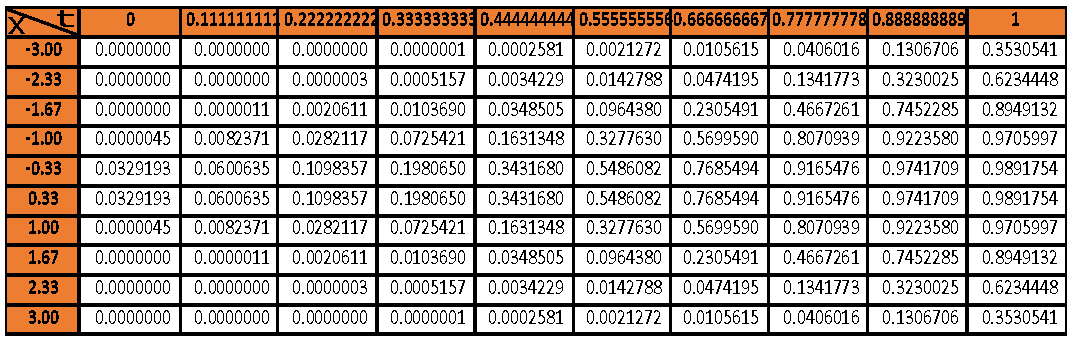
\includegraphics[scale=0.9]{simulacion/tablad1.pdf}
					\caption{{\footnotesize Tabla de iteraciones obtenidas con Matlab para $d=1$ y $\rho =10$}}
				\end{figure}
	\item Para $d=10$. Consideramos $n=99$, luego introducimos la siguiente expresión en Matlab $w=\text{FKi}(-3,3,0,1,9,99,10,10)$
				\begin{figure}[H]
					\centering
					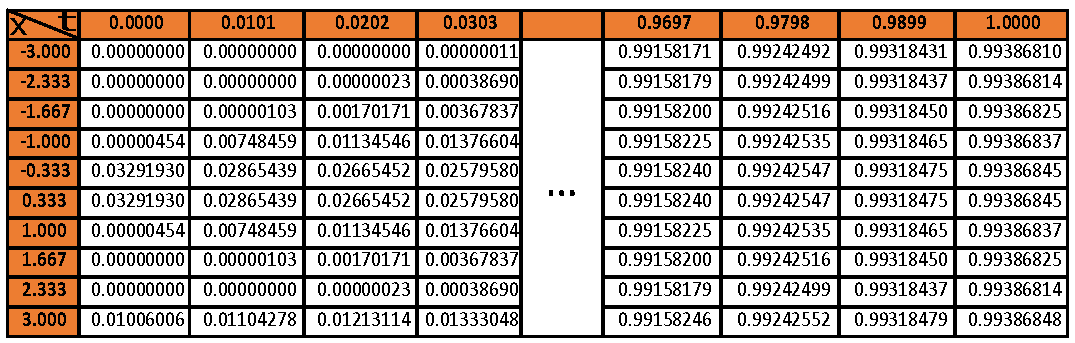
\includegraphics[scale=0.9]{simulacion/tablad10.pdf}
					\caption{{\footnotesize Tabla de iteraciones obtenida con Matlab para $d=10$ y $\rho =10$}}
				\end{figure}
	\item También podemos observar sus gráficas
				\begin{figure}[h]
					\centering
					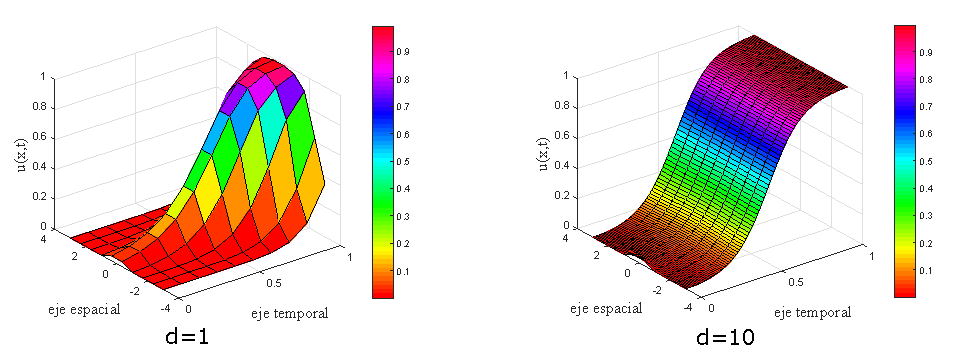
\includegraphics[scale=1]{simulacion/graficodeD.pdf}
					\caption{{\footnotesize Solución para un parámetro de difusión muy pequeña en la izquierda y una difusión grande en la derecha}}
					\label{figuraD}
				\end{figure}
	
\end{enumerate}

\subsubsection{Es constante el coeficiente $d$ de difusión}
Supondremos que $d=10$ permanece constante:

\begin{enumerate}
	\item Para $\rho=0\mbox{.}1$. Consideramos $n=69$, luego introducimos la siguiente expresión en Matlab $w=\text{FKi}(-3,3,0,1,9,69,10,0\mbox{.}1)$
	\begin{figure}[H]
		\centering
		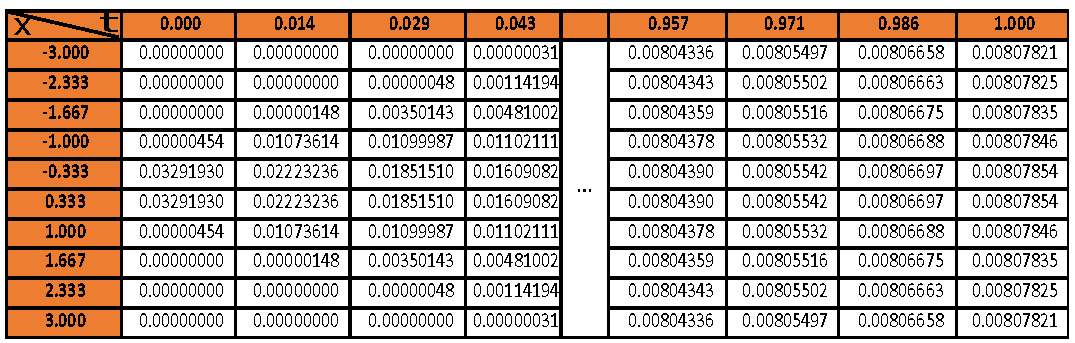
\includegraphics[scale=0.9]{simulacion/tabladrho01.pdf}
		\caption{{\footnotesize Tabla de iteraciones obtenida con Matlab para $d=10$ y $\rho =0\mbox{.}1$}}
	\end{figure}
	\item Pra $\rho=100$. Consideramos $n=99$, luego introducimos la siguiente expresión en Matlab $w=\text{FKi}(-3,3,0,1,9,99,10,100)$
		\begin{figure}[H]
			\centering
			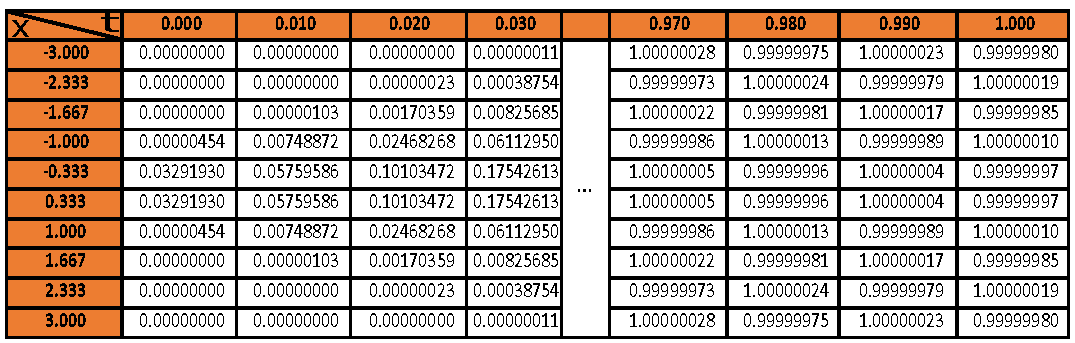
\includegraphics[scale=0.9]{simulacion/tabladrho100.pdf}
			\caption{{\footnotesize Tabla de iteraciones obtenida con Matlab para $d=10$ y $\rho =100$}}
		\end{figure}
	\item También podemos observar sus gráficas 
		\begin{figure}[H]
			\centering
			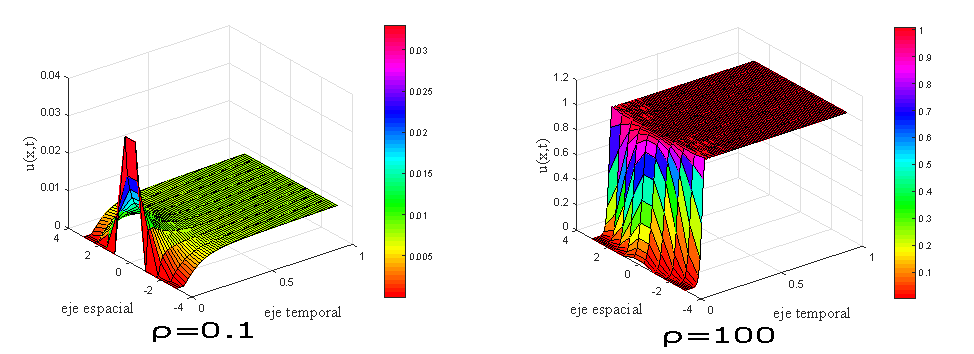
\includegraphics[scale=1]{simulacion/graficoderho.pdf}
			\caption{{\footnotesize Solución para un parámetro de proliferación muy pequeña en la izquierda y una proliferación elevada en la derecha}}
			\label{figuraparaRHO}
		\end{figure}
\end{enumerate}
 


		\chapter{Conclusión}
		%%%%%%%%%%%%%%%%%%%%%%%%%%%%%%%%%%%%%%%%%%%%%%%%%%%%%%%%%%%%%%%
\section{Cuando el parámetro $\rho$ de proliferación es constante }
	Analizar las tablas puede resultar tedioso por podemos analizar las gráficas de la Figura \ref{figuraD}.\\

	Se observa  que independientemente del los valores asignados al coeficiente de difusión ambos modelos muestran que en el periodo de un año llegan  a ocupar el máximo del tejido. (Recordar que $u$ se tomo en su forma normalizada).\\
	
	Por el contrario, se ve que cuando el coeficiente de difusión es significativa el número de células se expande en un periodo muy breve  de tiempo cubriendo todo el eje espacial; sin embargo, cuando $d$ es pequeño no la cubre incluso cuando $u=1$ (en máximo al cabo de un año).
	
\section{Cuando el coeficiente $d$ de difusión es constante}
	
	Para este caso analizaremos la Figura \ref{figuraparaRHO} \\
	
	Lo primero que notamos es que en ambos modelos el tumor cubre casi instantáneamente  todo el eje espacial.\\
	
	Si nos fijamos en el parámetro de difusión notaremos que para $rho=0.1$ a pesar de que se difunde rápidamente  apenas cubre la capacidad del tejido quedándose a lo largo del año  en $U=0.008$ en promedio. Sin embargo, para $rho=100$, un valor muy alto de proliferación, no solo se difunde rápidamente, sino que  además en apenas poco tiempo el tumor ya ha cubierto el máximo del tejido siendo este $u=1$.
		\backmatter
		\chapter{Anexo}
		%%%%%%%%%%%%%%%%%%%%%%%%%%%%%%%%%%%%%%%%%%%%%%%%%%%%%%%%%%%%%%%%%%%%%%%%%%%%%%%%%%%%%%%%%%%%%%%%%%%%%%%%%%%%%%%%%%%%%%%%
\section*{Fórmulas de aproximación}

Las aproximaciones de las derivadas de primer y segundo orden generalmente son resueltas mediante diferencias finitas, siendo estas las aproximaciones que se toman a las derivadas ya mencionadas por fórmulas como consecuencia de la fórmula de Taylor y de la interpolación por polinomios de Lagrange.\\
	
		Primero se hace una partición del dominio, partición que primero se aplica al intervalo $\left[a,b\right]$ \textit{del eje espacial}, de forma regular con tamaño de paso $h$ y luego al  intervalo $\left[0,T\right]$ del \textit{eje temporal}, de forma regular con tamaño de paso $k$.\\
		
		Con ello las aproximaciones por \textit{diferencias finitas} que vamos a usar para las derivadas parciales de la función $u=u(x,t)$ son:\\
		
		\textbf{Fórmula de dos puntos:}
		\begin{center}
			$$\frac{ \partial u({ x }_{ i },{ t }_{ j }) }{ \partial t } \approx \frac { u({ x }_{ i },{ t }_{ j+1 })-u({ x }_{ i },{ t }_{ j }) }{ k }$$ (\textit{Progresiva})\\
			
			$$\frac{ \partial u({ x }_{ i },{ t }_{ j }) }{ \partial t } \approx \frac { u({ x }_{ i },{ t }_{ j })-u({ x }_{ i },{ t }_{ j-1 }) }{ k }$$ (\textit{Regresiva})\\
			
			$$\frac{ \partial u({ x }_{ i },{ t }_{ j }) }{ \partial t } \approx \frac{1}{2}\frac { u({ x }_{ i },{ t }_{ j+1 })-u({ x }_{ i },{ t }_{ j-1 }) }{ k }$$ (\textit{Centrada})
			
		\end{center}
	
		\par \textbf{Fórmula de tres puntos - centradas:}
		\begin{center}
			$$\frac{ \partial^2 u({ x }_{ i },{ t }_{ j }) }{ \partial t^2 } \approx \frac { u({ x }_{ i },{ t }_{ j+1 })-2u({ x }_{ i },{ t }_{ j }) + u({ x }_{ i },{ t }_{ j-1 })}{ k^2 }$$
			$$\frac{ \partial^2 u({ x }_{ i },{ t }_{ j }) }{ \partial x^2 } \approx \frac { u({ x }_{ i+1 },{ t }_{ j })-2u({ x }_{ i },{ t }_{ j }) + u({ x }_{ i-1 },{ t }_{ j })}{ h^2 }$$
		\end{center}
%%%%%%%%%%%%%%%%%%%%%%%%%%%%%%%%%%%%%%%%%%%%%%%%%%%%%%%%%%%%%%%%%%%%%%%%%%%%%%%%%%%%%%%%%%%%%%%%%%%%%%%%%%%%%%%%%%%%%%%%%%%%%%%
\section*{Desigualdad de Gronwall }

Sea $I$ un intervalo de la forma $[a,b]$ con $a<b$. Si $u$ es diferenciable en $I$ y satisface $u'(t)\leq \beta(t)u(t)$ entonces se cumple:

$$ u(t)\leq u(a)exp\left(\int_{a}^{t}\beta(s)ds\right)$$

		\chapter{Bibliografía}
		\begin{enumerate}
		\item Modelos matemáticos de competición entre cáncer y sistema inmune. Trabajo Fin de Grado de José García Otero; Leioa, 21 de febrero de 2019.
		\item Jaime G. de la Garza Salazar \& Paula Juárez Sánchez (2014). \textit{El Cáncer}. Universidad Autónoma de Nuevo León. Monterrey, México.
		\item Jorge Rodríguez. El modelo logístico: \textit{Una alternativa para el estudio del crecimiento poblacional de organismos}. Universidad Autónoma de Nayarit, México.
		\item Guillermo Abramson. \textit{La matemática de los sistemas biológicos}. Universidad Nacional de Cuyo, Argentina.
		\item Clara Rodriguez. \textit{Aplicación de procesos de control óptimo y optimización en la evolución de modelos tumorales}. Universidad de Castilla - La Mancha, España.
		\item \url{https://acortar.link/tfrA6}
		\item \url{https://acortar.link/HGXlX}
	\end{enumerate}
\end{document}